\documentclass[notitlepage]{report}

\usepackage[utf8]{inputenc}
\usepackage[T1]{fontenc}
\usepackage[german]{babel}
\usepackage{hyperref}
\usepackage{amsmath}
\usepackage{graphicx}
\usepackage{siunitx}
\usepackage{arydshln}	%needs to be below siunitx
\usepackage{upgreek}
\usepackage{svg}

\sisetup{per-mode=fraction}
\sisetup{retain-explicit-plus}

\title{Ex4 - Zusammenfassung}
\author{Martin Pittermann}

\newcommand*{\corresponds}{\mathrel{\widehat=}}
\newcommand*\textmath[1]{\ensuremath{\mathrm{#1}}}

\begin{document}
\maketitle
\begin{abstract}
	...weil die Vorlesung einfach nichts taugt.\\
\end{abstract}

\chapter{Atomphysik}
\section{Konstanten}
\bgroup
\def\arraystretch{1.5}
\begin{tabular}{l|l}
	$\alpha = \frac{1}{4 \uppi \epsilon_0} \cdot \frac{\text{e}^2}{\hbar c} \approx \frac{1}{137}$&	Sommerfeld'sche Feinstrukturkonstante\\
	\hdashline
	$R_\infty = \frac{m_\text{e} \text{e}^4}{8 \epsilon_0^2 h^3 c} \approx \SI{1.097e7}{\per\meter} \corresponds \SI{13.6}{\eV}$&	Rydbergkonstante\\
\end{tabular}
\egroup

\section{Quantenzahlen}

\bgroup
\def\arraystretch{1.5}
\begin{tabular}{l|c|l|l}
	QZ&
	Einstellmögl.&
	assoz. Drehimpuls&
	Beschreibung\\
	\hline
	$n = 0 \dots$&&&\\
	\hdashline
	$l = 0 \dots (n-1)$&&	$|\vec{l}| = \hbar \sqrt{l(l+1)}$&Bahndrehimpuls\\
	$m_l = -l \dots l$&[$2l + 1$]&	$\vec{l}_z = \hbar m_l$&\\
	&&$\vec{L} = \sum \vec{l}$&Gesamtbahndrehimpuls\\
	\hdashline
	$s = \frac{1}{2}$ (Fermionen)&&		$|\vec{s}| = \hbar \sqrt{s(s+1)}$&	Spin\\
	$m_s = -s \dots s$&[$2$]&		$\vec{s}_z = \hbar m_s$&\\
	&&$\vec{S} = \sum \vec{s}$&Gesamtspin\\
	\hdashline
	$j = |l + m_s|$&&	$|\vec{j}| = \hbar \sqrt{j(j+1)}$&	Gesamtdrehimpuls (1$\text{e}^-$)\\
	&&$\vec{j} = \vec{l} + \vec{s}$&\\
	$m_j = -j \dots j$&[$2j + 1$]&		$\vec{j}_z = \hbar m_j$&\\
	&&$\vec{J} = \sum \vec{j}$&Gesamthüllendrehimpus\\
	\hdashline
	$I = \frac{1}{2}, 1 \dots$&[siehe \autoref{sec:kernspin}]&	$|\vec{I}| = \hbar \sqrt{I(I+1)}$&	Kerndrehimpuls\\
	$m_I = -I \dots I$&&		$\vec{I}_z = \hbar m_I$&\\
	\hdashline
	$F = |J-I| \dots J+I$&[$2\min\{I,J\} + 1$]&	$|\vec{F}| = \hbar \sqrt{F(F+1)}$&	Gesamtdrehimpuls Atom\\
	&&$\vec{F} = \vec{J} + \vec{I}$&\\
\end{tabular}
\egroup

\section{Magnetisches Moment}
Ein Drehimpuls erzeugt immer ein magnetisches Moment.\\
Für den Bahndrehimpuls eines Elektrons gilt
\begin{equation*}
\vec{\mu_l}
= -g_l \cdot \mu_\text{B} \cdot \frac{\vec{l}}{\hbar}
= - \mu_\text{B} \cdot \frac{\vec{l}}{\hbar} \qquad (g_l = 1),
\end{equation*}
für den Spin eines Teilchens x gilt:
\begin{equation*}
\vec{\mu_s} = g_\text{x} \cdot \mu_\text{x} \cdot \frac{\vec{s}}{\hbar}
\end{equation*}
mit $\mu_\text{x} = \frac{\text{e}}{2 m_\text{x}}$ und den g-Faktoren
\begin{center}
\begin{tabular}{ll}
	Elektron&	$g_\text{e} \approx \num{-2.002}$\\
	Neutron&	$g_\text{n} \approx \num{-3.826}$\\
	Proton&	$g_\text{p} \approx \num{+5.586}$\\
\end{tabular}
\end{center}
g-Faktoren von ganzen Atomkernen werden experimentell bestimmt, dabei wird $\vec{s}$ durch $\vec{I}$ ersetzt.

\section{Kernspin}\label{sec:kernspin}
Der Kernspin $I$ ist die Summe der Bahndrehimpulse und Spins der Nukleonen.
Bei Kernen mit mehreren Nukleonen bilden je zwei Protonen/Neutronen ein Paar mit Gesamtdrehimpuls $\vec{I} = 0$.\\
Daher gilt für den Kernspin $\vec{I} = \sum (\vec{s_i} + \vec{l_i})$ eines Kerns mit Nukleonenzahl $A$:
\begin{center}
\bgroup
\def\arraystretch{1.25}
\begin{tabular}{lll}
	$A$ gerade&	gg&	$I = 0$\\
	&	uu&	$I = 0,1,\dots$ (zwei ungepaarte $\tfrac{1}{2}$-Spins)\\
	$A$ ungerade&	gu/ug&	$I = \tfrac{1}{2},\tfrac{3}{2},\dots$ (ein ungepaarter $\tfrac{1}{2}$-Spins)\\
\end{tabular}
\egroup
\end{center}
, wobei gg/ug/uu je für eine gerade/ungerade Anzahl an Protonen und Neutronen steht.

\section{Energieniveaus H-Atom}
\begin{center}
	\includegraphics[width=.8\linewidth]{img/energieniveaus}\\
	(Energie nicht maßstabsgetreu)
\end{center}

\subsection{Bohr}
\begin{equation*}
	E_n = -h \, c \, R_\infty \frac{1}{n^2}
\end{equation*}
$R_\infty$ proportional zu $m_\text{e}$, ersetze $m_\text{e}$ durch reduzierte Masse oder zB. Myonenmasse.

\subsection{Dirac (Spin-Bahn-Kopplung)}
Wechselwirkung zwischen Spin- und Bahnmagnetismus:
\begin{equation*}
	V_{ls} = -\vec{\mu_s} \cdot \vec{B_l}
\end{equation*}
Aus $\vec{j} = \vec{l} + \vec{s}$ und Quantisierung $|\vec{j}| = \hbar \sqrt{j(j+1)}$ etc folgt
\begin{equation*}
	\vec{l} \cdot \vec{s} = \hbar^2 \tfrac{1}{2}\left(j(j+1)-l(l+1)-s(s+1)\right)
\end{equation*}
Ergibt (incl. relativistischer Effekte)
\begin{equation*}
	E_{nj} = E_n \left(1 + \frac{Z^2 \alpha^2}{n^2} \cdot \left(\frac{n}{j+\frac{1}{2}} - \frac{3}{4} \right)\right)
\end{equation*}
und liefert stets negative Verschiebung (da $E_n$ negativ), also eine stärkere Bindung.

\subsection{Lamb-Shift}
Wechselwirkung mit virtuellen Elektron-Positron Paaren heben Entartung von Zuständen mit gleichem j auf.

\subsection{Hyperfeinstruktur}
Wechselwirkung Kernspin - Bahndrehimpuls:
\begin{equation*}
	V_\text{HFS} = g_I \, \mu_\text{N} \, B_J \, \frac{\left[F(F+1)-I(I+1)-L(L+1)\right]}{2 \sqrt{J(J+1)}}
\end{equation*}
mit Bahnmagnetismus $B_J$.
Genaue Vorfaktoren werden experimentell bestimmt.

\section{Externen Felder}
\subsection{Drehimpulspräzession}
Bei vorhandener Quantisierungsachse (oBdA z-Achse) präzedieren Drehimpulse um ihre z-Komponente bzw bei zusammengesetzten Drehimpulsen, zB. $\vec{j} = \vec{l} + \vec{s}$ präzedieren die einzelnen Drehimpulse um den Gesamtdrehimpuls, dieser präzediert um seine z-Komponente.
Die Präzessionsfrequenz ist gegeben durch die Lamourfrequenz
\begin{equation*}
	\omega_\text{L} = \frac{\mu}{\hbar} \cdot g \cdot B_\text{ext}
\end{equation*}

\subsection{Zeemann Effekt}
Der Drehimpuls der Hülle wechselwirkt mit einem externen Magnetfeld
\begin{equation*}
	V_\text{Ze} = - \, \vec{\mu} \cdot \vec{B}_\text{ext} = - \, \mu \, m_J \cdot B_\text{ext}.
\end{equation*}

Der \textbf{normaler Zeemann Effekt} tritt auf wenn kein Gesamtspin vorliegt, jedes Energieniveau $L$ spaltet auf in $2L + 1$ ($L = \sum l$) Äquidistante Niveaus mit $\Delta E = \hbar \omega_\text{L} = (g_L \cdot) \mu_L B_\text{ext}$, unabh. von L.

Beim \textbf{anomalen Zeemann Effekt} tritt zusätzlich Spinmagnetismus auf. Es erfolgt eine Aufspaltung des $J$-Niveau in $2J + 1$ Niveaus, die wegen den unterschiedlichen $g$-Faktoren von Spin und Bahndrehimpuls abhängig von $J$ sind.

\subsection{Kernspinresonanz}

Äquivalent zum Zeemann Effekt, mit Kernmagneton:
\begin{align*}
	V_\text{pot} &= \underbrace{g_l \, \mu_N \, B_\text{ext}}_{|\Delta E|} \cdot m_I\\
	\rightarrow \omega &= g_l \, \mu_N \, B_\text{ext} = \omega_\text{L}
\end{align*}
Die Übergänge zwischen den neuen Energieniveaus können nur mit der Resonanzfrequenz $\omega$ angeregt werden.

\subsection{Stark-Effekt}

Wechselwirkung des elektrischen Dipols eines Atoms mit einem externen Magnetfeld, Energieshift proportional zu $E$ und $|m_J|$.
Es kann auch ein Dipolmoment induziert werden (Polarisation des Atoms) $\rightarrow \; \propto E^2$.

\section{Mehrelektronensysteme}
\subsection{Paulisches Ausschließungsprinzip}
Ausschließungsprinzip: zwei Elektronen in einem Atom können nicht in allen Quantenzahlen übereinstimmen.
$\rightarrow$ Spins in gleichen Orbitalen sind antiparallel.

Bei entarteten Sternen: gilt Pauli für ein Phasenraumvolumen $dr^3 \cdot dp^3 \, = \, h^3$.

\subsection{Beschreibung von Zuständen}
\begin{equation*}
	n^{2S+1}L_j
\end{equation*}
\begin{itemize}
	\item $L = \sum l, \; S = \sum s$: Gesamtbahndrehimpuls / Spin
	\item ($2S + 1$): Spin-Multiplizität (Anzahl Einstellmöglichkeiten für Gesamtspin)
\end{itemize}
Pauli: $S = 0$ für $L = 0$ (S-Orbital)

\subsection{Kopplung von Drehimpulsen}
\begin{center}
	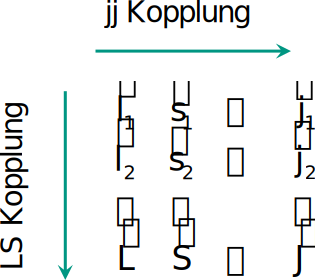
\includegraphics[width=.25\textwidth]{img/ls-jj-coupling.pdf}
\end{center}

\subsubsection{Russel-Saunders ($LS$)-Kopplung}
Tritt bei kleinen Kernen ($Z < 30$) auf.

\[\vec{S} = \sum \vec{s}, \quad \vec{L} = \sum \vec{l}, \quad \vec{J} = \vec{L} + \vec{S}\]

Quantisierung bei zwei Elektronen ($\vec{l_1}$ und $\vec{l_2}$ nicht parallel): \[L = l_1 - l_2 \dots l_1 + l_2 \; (l_1 > l_2)\]

$\rightarrow$ $L=0$: S-Term, $L=1$: P-Term, $L=2$: D-Term.
\subsubsection{$jj$-Kopplung}

\subsection{Madelung Schema}
\begin{center}
\includegraphics[width=.25\textwidth]{img/madelung-rule.pdf}
\end{center}
In den jeweiligen Grundzuständen der Atome werden nach aufsteigendem $(n + l)$, zweitrangig nach aufsteigendem $n$ aufgefüllt.
Es gibt allerdings auch Ausnahmen wie zB. Chrom: \textmath{[Ar] 3d^5 4s^1}.


\end{document}
